% ------------------------------------------------------------------------------
% It describes the means used to manage a project.
% ------------------------------------------------------------------------------

\opt{never}{\addbibresource{03-tail/bibliography.bib}} % to make citation found in most IDE

\chapter{Project methodology}
\label{chap:methodology}

% -- Your text goes here --
This chapter covers all aspects of project management. A project plan is outlined, describing how the research was carried out. The Agile and \gls{kanban} methodologies are presented. Finally, the chapter concludes with a description of the management tools used and an account of the training received.

\minitoc
\newpage

% -----------------------------------------------------------------------------
\section{Project plan}

% -- Your text goes here --
At the start of the project, a research plan was drawn up. It is presented in figure \ref{fig:work_packages} in the form of \glspl{work_package}.
\begin{center}
    \begingroup
    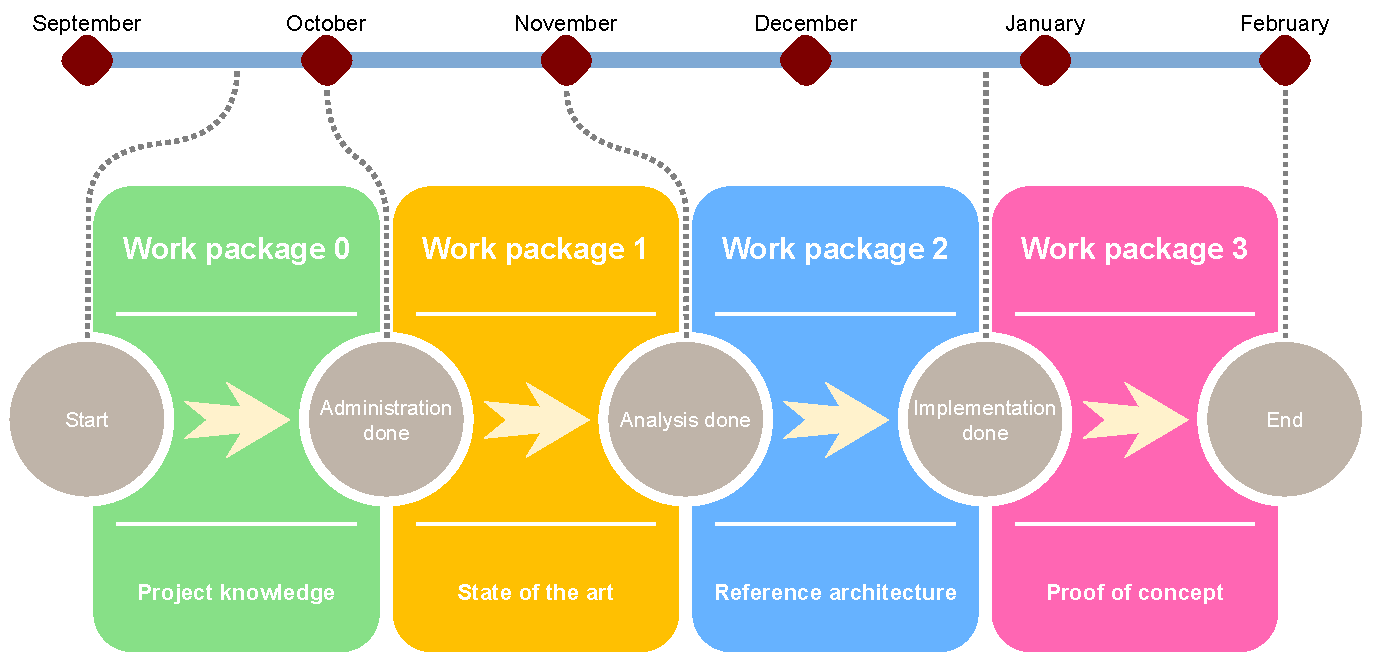
\includegraphics[width=1\columnwidth]{methodology/work_packages.pdf}
    \captionof{figure}{Project plan}
    \label{fig:work_packages}
    \endgroup
\end{center}
The first \gls{work_package} covers all administrative activities. The aim of this initial phase was to gain an in-depth understanding of the project, become aware of the issues and clearly define the specifications. It lasted around two weeks.

About a month was spent researching existing solutions that were closest to the project through a state of the art, involving consultation of scientific articles and other documentation.

The third \gls{work_package} focuses on the \gls{cloud_infrastructure}, with around two months dedicated to this implementation phase. This part includes the creation of the \acrshort{ci}/\acrshort{cd} process.

In the latest \gls{work_package}, completion of the reference architecture was scheduled with just over a month remaining. It is at this stage that the final functionalities are developed. This is also the phase when the whole package must undergo testing and validation before being released as open source on a shared repository.


% -----------------------------------------------------------------------------
\section{Research methodology}

% -- Your text goes here --
The research methodology adopted in this thesis began with a state of the art survey of the existing solutions most relevant to this project. Next, an overview of the reference architecture was established to facilitate implementation. A judicious choice of development tools was also made. In parallel, the implementation was carefully designed, followed by validation of the results through a proof of concept.

Throughout the process, agile methodology, in particular the \gls{scrum} method, was used, enabling iterative project management. Weekly meetings were scheduled with the professor responsible for the work, as well as with certain company staff on an optional basis. To ensure that the project progressed efficiently, the \gls{kanban} method was used. This approach uses virtual cards to represent each task, organised in a table to clearly track progress. It is also used to break the project down into smaller parts to more accurately estimate the time required throughout the process.


% ------------------------------------------------------------------------------
\section{Literature search}

% -- Your text goes here --
Literature search has focused on academic search engines. The following search engines were used :
\begin{itemize}
    \item \href{https://scholar.google.com}{Google Scholar}
    \item \href{https://ieeexplore.ieee.org/Xplore/home.jsp}{IEEE Xplore}
    \item \href{https://www.sciencedirect.com}{ScienceDirect}
\end{itemize}
The sources were mainly conference papers. Some information was found on websites. The following keywords were used to find sources that met the requirements of this analysis:
\begin{itemize}
    \item integration
    \item reference architecture
    \item embedded systems
    \item \acrshort{iot}
    \item \nameref{subsec:cloudnative}
    \item \gls{cloud}
    \item \hyperref[subsec:cloudcomputing]{cloud computing}
    \item \gls{cloud} providers
    \item \gls{cloud} platforms
    \item \acrlong{iac}
    \item \acrshort{iac} tools
    \item \nameref{sec:arm_systemready}
\end{itemize}


% ------------------------------------------------------------------------------
\section{Agile methodology}

% -- Your text goes here --
Agile methodology is the main project management method used in this work. It enables the project to be managed from the specifications to the final product. The idea for this method was conceived in the 70s or even before \cite{abbas_historical_2008}.  The idea was to change the development process in software engineering by using iterative techniques. Traditional methods worked with sequential techniques, often called Waterfall. Figure \ref{fig:waterfall_vs_scrum} shows the difference between these two approaches.
\begin{center}
    \begingroup
    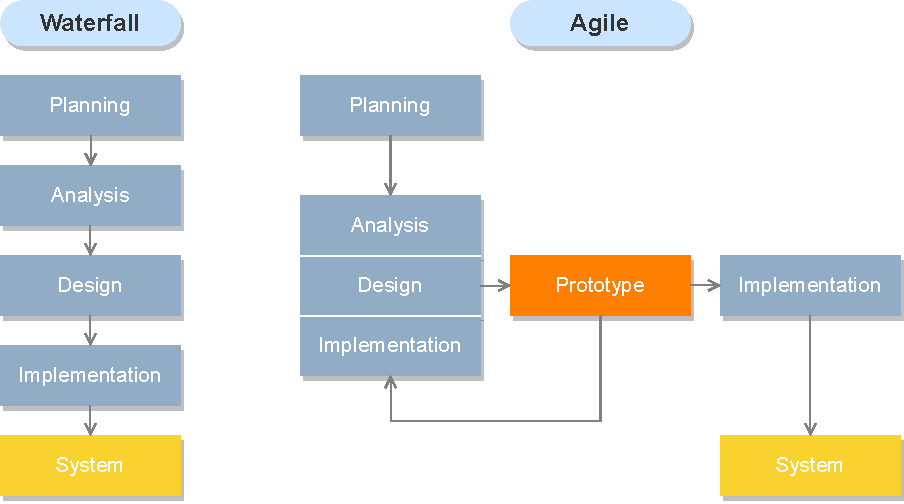
\includegraphics[width=1\columnwidth]{methodology/waterfall_vs_scrum.pdf}
    \captionof{figure}{Sequential and iterative process \cite{course_MA_ITProMan}}
    \label{fig:waterfall_vs_scrum}
    \endgroup
\end{center}
The Waterfall methodology is considered cumbersome. There are deliverables after each phase. Approval is required before moving on to the next phase. It is difficult to go backwards (by moving up the phases). Professors explained this very well during a Masters course given at the \gls{hes} \cite{course_MA_ITProMan}. They added that this method is best used in very large projects where it is difficult to split teams into small groups to work iteratively.

These same teachers \cite{course_MA_ITProMan} described the agile methodology as follows:
\begin{quote}
    \textit{"AGILE" is about values and principles, not practices, but many practices support them. It's not about doing agile, it's about being agile}.
\end{quote}
Several agile process frameworks were created before the 2000s. Examples include \gls{scrum}, XP, RUP, etc. Between the 11th and the 13th of February 2001, 17 people from these different frameworks met to find an alternative to cumbersome, documentation-driven software development processes. They created the agile software development manifesto \cite{manifesto_agile} :
\begin{itemize}
    \item[] \textit{Individuals and interactions over processes and tools}
    \item[] \textit{Working software over comprehensive documentation}
    \item[] \textit{Customer collaboration over contract negotiation}
    \item[] \textit{Responding to change over following a plan}
\end{itemize}
The central principle of agile is to have very rapid iterations to build the first business values. The customer is at the centre of the process thanks to frequent communication with the development team \cite{course_MA_ITProMan}. The process framework chosen for this project is \gls{scrum}. It is very well suited to small projects with small teams. It enables the first software prototypes to be delivered quickly. It adapts easily to changes, unlike a sequential method. It is also based on experience. The idea is to learn continuously through iterations. This is an important point in terms of learning from new developments in the project. This is one of the most popular agile methods. This approach was launched in 1995 by Ken Schwaber and Jeff Sutherland \cite{scrum_guide_site}.

\subsection{\Gls{scrum} roles}
Figure \ref{fig:scrum_roles} shows the different roles in a \gls{scrum} team.
\begin{center}
    \begingroup
    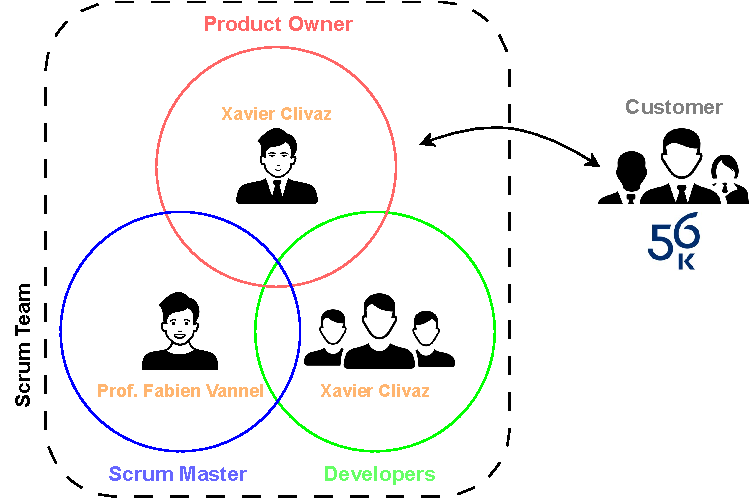
\includegraphics[width=.8\columnwidth]{methodology/scrum_roles.pdf}
    \captionof{figure}{\Gls{scrum} roles}
    \label{fig:scrum_roles}
    \endgroup
\end{center}
A \gls{scrum} guide has been written by Jeff Sutherland and Ken Schwaber to explain the rules \cite{scrum_guide}. First of all, there is the \acrfull{po}. This is the customer's spokesperson. It is he who defines the product's functionalities. They are recorded in a Product Backlog in the form of tasks. He must manage these tasks by prioritising some of them. He is also responsible for the value and return on investment (\acrshort{roi}) of the product. The development team is generally a small one (around seven people \cite{course_MA_ITProMan}). It is capable of self-management. There are no specific roles or positions. Developers have to deal with tasks that are chosen from the Sprint Backlog. Finally, the \gls{scrum} Master is required to be of service to the team. He accompanies the team of developers and prevents obstacles from getting in the way of progress. It is the \gls{scrum} Master who establishes the practices and rules of \gls{scrum}.

\subsection{\texorpdfstring{\gls{scrum}}{} process}
The \gls{scrum} process is relatively simple. It follows the theory described in the official \gls{scrum} guide \cite{scrum_guide}. The life cycle is shown in figure \ref{fig:scrum_process}.
\begin{center}
    \begingroup
    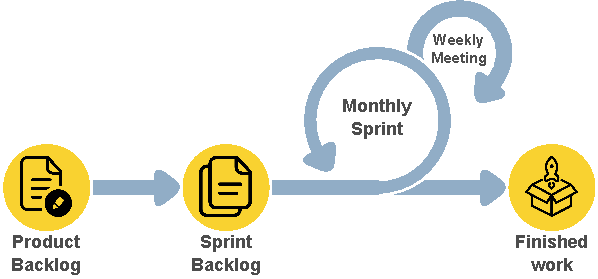
\includegraphics[width=.9\columnwidth]{methodology/scrum_process.pdf}
    \captionof{figure}{\Gls{scrum} life cycle}
    \label{fig:scrum_process}
    \endgroup
\end{center}
The process is made up of multiple elements. It begins on the left of the diagram with the Product Backlog. This is a backlog that is filled by the \acrshort{po}. Since the Product Backlog is generally filled with many functionalities divided into tasks, only one part needs to be selected to be placed in the Sprint Backlog. A Sprint generally corresponds to a period of one month during which the tasks in the Sprint Backlog must be completed. During a Sprint, team meetings are organised every day. These are called Daily Meetings and usually last 15 minutes. A Daily Meeting ensures that, at least once a day, the entire team is available to get support on any problems encountered. In this project, only weekly meetings are held, depending on the distance separating the \gls{scrum} Master and the team of developers. Before each Sprint, a Sprint Planning is carried out to determine the tasks from the Product Backlog to be put into the Sprint Backlog. At the end of a Sprint, an inspection is made of how the Sprint went, with the aim of improving quality and efficiency. This is called a Sprint Retrospective. Finally, it's important to remember that at the end of each Sprint, one stage of the final product is completed. Sometimes this is called an increment.

% ------------------------------------------------------------------------------
\section{KanBan methodology}

% -- Your text goes here --
The \gls{kanban} methodology is very well integrated into \gls{scrum}. Its aim is to manage the workflow as efficiently as possible. According to the \gls{kanban} guide produced by \gls{scrum}.org \cite{kanban_guide}, several fundamental metrics should be taken into account for the flow:
\begin{itemize}
    \item \textbf{\acrfull{wip}} : the number of tasks/items started and not completed.
    \item \textbf{Cycle Time} : the time elapsed between the start and end of a task.
    \item \textbf{Work Item Age} : the time elapsed between the start of the task and now.
    \item \textbf{Throughput} : the number of tasks completed per unit of time.
\end{itemize}
The average cycle time can be predicted using Little's Law \cite{little_law}:
\begin{equation}
    average\ cycle\ time = \frac{average\ \acrshort{wip}}{average\ throughput}
\end{equation}
It explains that the more tasks there are in progress, the longer it will take to complete them. A cycle time in \gls{kanban} can be correlated to a Sprint in the \gls{scrum} methodology. Using this methodology, it is therefore possible to define the right number of tasks for each Sprint Planning. Note that the more you divide a feature into smaller tasks, the easier it will be to predict the cycle time.

\gls{kanban} does more than just limit the \acrshort{wip}. It provides a transparent display of the workflow. Tasks can be represented in a table, as shown in figure \ref{fig:kanban_example}. In this case, the table is virtual and can be viewed from anywhere by the whole \gls{scrum} team.
\begin{center}
    \begingroup
    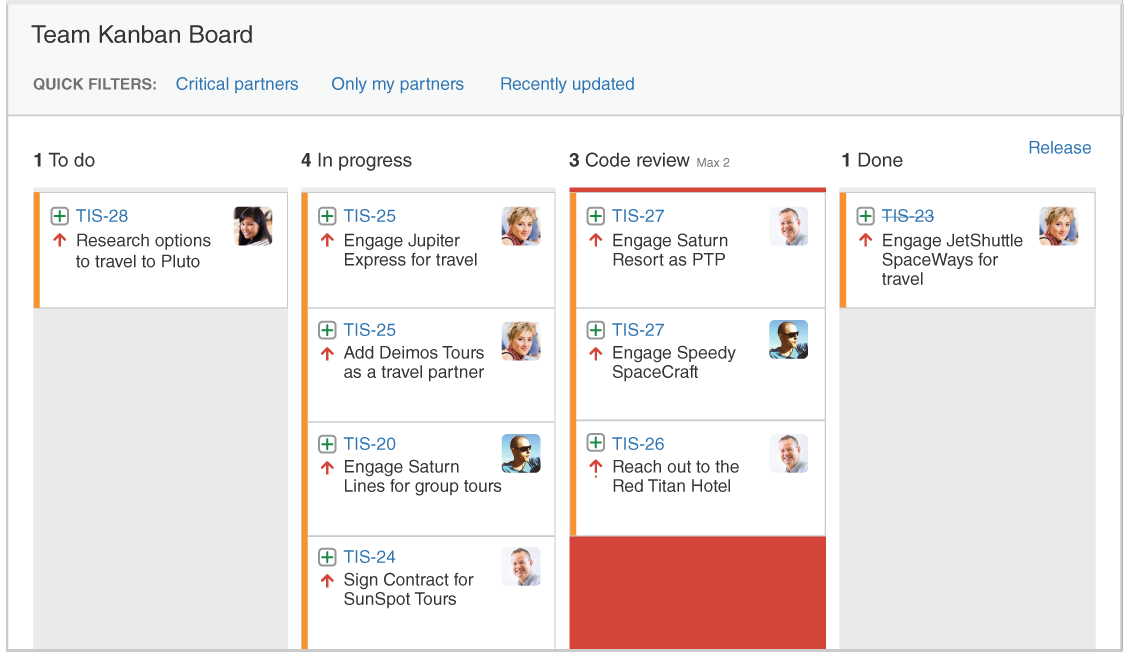
\includegraphics[width=1\columnwidth]{methodology/kanban_example.png}
    \captionof{figure}{Example of a virtual \gls{kanban} table \cite{kanban_example}}
    \label{fig:kanban_example}
    \endgroup
\end{center}
Each label in the table corresponds to a task. A task can contain a priority level and is often assigned to a member of the \gls{scrum} team. All this is defined during Sprint Planning. The labels are categorised in columns to show their progress.


% ------------------------------------------------------------------------------
\section{Project management tools}

% -- Your text goes here --
\subsection{Version management}
Version management, embodied by tools such as Git, remains an essential part of the software development ecosystem. This practice offers a structured approach to tracking and maintaining changes to a project's code. One of the major benefits lies in its ability to keep a complete history of changes, facilitating collaboration between team members working on the same project.
\begin{center}
    \begingroup
    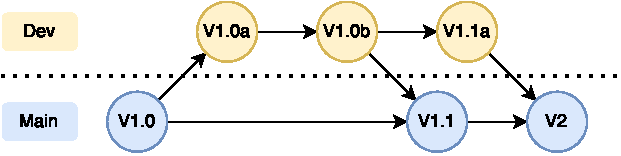
\includegraphics[width=0.8\columnwidth]{methodology/version_control.pdf}
    \captionof{figure}{Example of version management with two branches}
    \label{fig:version_control}
    \endgroup
\end{center}
An example of a visual representation of a project is shown in figure \ref{fig:version_control}, comprising several distinct versions and branches. Branches allow developers to work on alternative versions of the source code, facilitating parallel development, feature isolation and efficient change management without affecting the main branch.

When part of the development is considered complete, it becomes common practice to create a new version. This version freezes the current state of the project at a specific point in time, providing a clear and stable reference. This ability to create versions means that it is possible to return to previous states of the project if problems arise, whether identified by members of the development team or by external stakeholders, such as customers.

In short, version management, embodied by Git, transcends its simple function of tracking changes to become a central pillar of collaborative working, risk management and preserving the integrity of a software project. Its widespread adoption across the industry is testament to its continuing importance in delivering robust, scalable software development projects.

\subsection{\acrfull{ci} and \acrfull{cd}}
\acrshort{ci}/\acrshort{cd} (\acrlong{ci}/\acrlong{cd}) integrates synergistically with version management, and in particular with the \acrshort{devops} framework, as illustrated in figure \ref{fig:devops}. The aim of the \acrshort{devops} method is to automate software development processes, thereby encouraging collaboration between development teams (grey area) and operational teams (pink area). Two major components of \acrshort{ci}/\acrshort{cd} have emerged from this approach, namely \acrfull{ci} and \acrfull{cd}, which have become fundamental pillars for developers.
\begin{center}
    \begingroup
    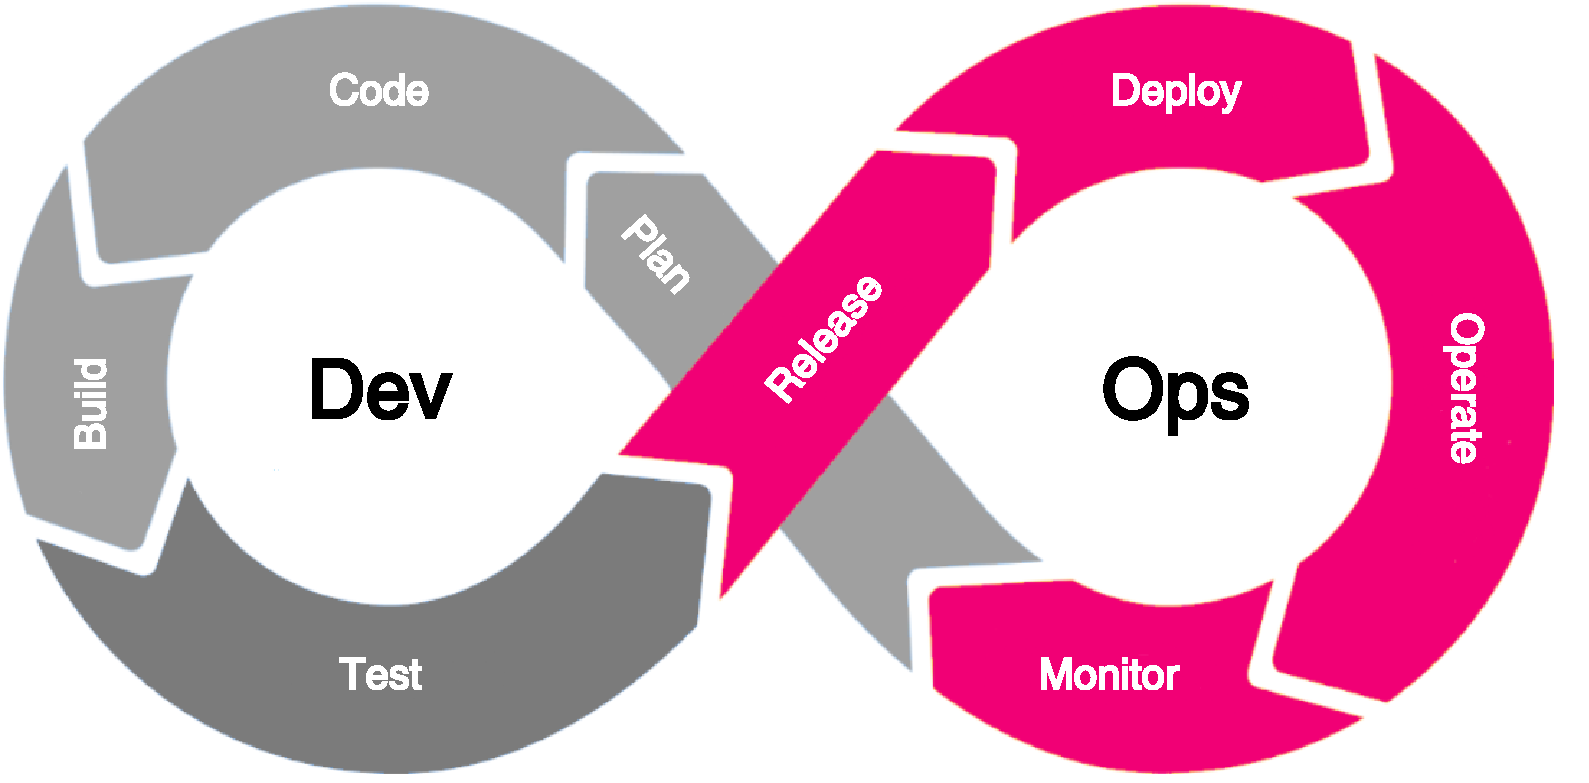
\includegraphics[width=0.75\columnwidth]{methodology/devops.pdf}
    \captionof{figure}{\gls{devops} method}
    \label{fig:devops}
    \endgroup
\end{center}
\acrshort{ci} involves automating various processes with each new software release. These processes typically include building, testing and deploying the software design, as shown in figure \ref{fig:devops}. The main motivation for inventing the \acrshort{ci} was to reduce the time needed between launching a project and bringing it to market, a concept known as time-to-market. This automation takes advantage of the constant evolution of machines, contrasting with the physical and moral limits of human beings. The benefits of \acrshort{ci} also extend to team collaboration, simplified debugging, reduced costs, improved software quality, and much more.

\acrshort{cd} goes hand in hand with the \acrshort{ci}, aimed at automating the deployment of software to production environments. It eliminates the tedious manual steps associated with deployment, ensuring fast, reliable and frequent delivery of new features and software updates.

\acrshort{ci}/\acrshort{cd} represents a modern and essential approach to the software development lifecycle, offering efficiency gains, improved team collaboration, accelerated time-to-market and an overall improvement in the quality of software products.

\subsection{\Glspl{work_package}}
\Glspl{work_package} are specific, delimited elements of a project which are assigned to a team or an individual for completion. Each \gls{work_package} represents a well-defined task or set of tasks, often associated with concrete deliverables. They facilitate the management and monitoring of the project by allowing a clear division of responsibilities and helping to assess progress. In short, \glspl{work_package} are manageable units that contribute to the achievement of an overall project.

% ------------------------------------------------------------------------------
\section{Training}

% -- Your text goes here --
\subsection{\gls{aws} Certified \Gls{cloud} Practitioner}
\gls{aws} offers a number of certifications designed to validate the skills and knowledge of IT professionals working on the \gls{aws} platform. These certifications are designed to cover a variety of areas, from cloud architecture and operations management to security, databases, application development and more.

These certifications are widely recognised in the industry and can help professionals demonstrate their skills and progress in their \gls{cloud} careers. It is important to note that the \gls{aws} certification programme is evolving, and new certifications may be added as new services and features are introduced to the \gls{aws} platform.

The certification achieved as part of this project was as follows : \textbf{\gls{aws} Certified \Gls{cloud} Practitioner}. This is the first certification to give a general overview of a \gls{cloud} platform to professionals with no previous experience in this field. \gls{aws} defines it as follows :
\begin{quote}
    \textit{The \gls{aws} Certified \Gls{cloud} Practitioner validates foundational, high-level understanding of \gls{aws} \Gls{cloud}, services, and terminology.  This is a good starting point on the \gls{aws} Certification journey for individuals with no prior IT or \gls{cloud} experience switching to a \gls{cloud} career or for line-of-business employees looking for foundational cloud literacy. \cite{aws_practitioner_certificate}}\\
\end{quote}
Online lessons were taken at the start of the project and, within a month, an official exam was successfully passed.
\begin{center}
    \begingroup
    
\includegraphics[width=0.2\columnwidth]{methodology/aws_practitioner_certificate.png}
    \captionof{figure}{\gls{aws} Certified \Gls{cloud} Practitioner}
    \label{fig:aws_practitioner_certificate}
    \endgroup
\end{center}